\documentclass[../../main.tex]{subfiles}
\graphicspath{{\subfix{../../res/}}}
\begin{document}
From different literature review and papers, research seems to diverge and agree on different aspects. Making it difficult to pinpoint a specific variable that could point us in the direction of success prediction. From the country to institution itself, student history and background. It seems like choice has an important effect on whether a student may be successful in its study or not. However, we cannot satisfyingly say that choice makes student success.  Some outliers may have bad grades but be in reality a high potential success student. It all depends on a myriad of factors, which can be distilled into different variable that our \acrfull{ml} algorithms can learn from. We have to actually see and search (as we are going to do when looking at student dropout factors), which factors can be used to feed our models in order to correctly predict student success and find these outliers within the mass.\cite{kuh_what_2006, sa_how_2018}
We found these different point of view interesting to study for our future predictive model. These research have different conclusion on why students dropout from their studies, from an economical standpoint to a psychological one.\cite{opazo_analysis_2021} have found an interesting link with the study from\cite{spady_dropouts_1970} which found a correlation between the student dropout model and the social nature of suicide (\textit{social integration}), \cite{durkheim_suicide_1951}. This theory implies that the likelihood of suicide increase when there is an absence of : a)\textit{low normative congruence} and b)\textit{low friendship support}. Other literature from their state-of-the-art list these following as recurrent factors from multiple research\cite{opazo_analysis_2021,tinto_dropout_1975,caspersen_teachers_2015,lidia_problema_2006,bejarano_caso_2017,sinchi_acceso_2018,cavero_voluntad_2011,velasco_alisis_nodate}: 
\begin{itemize}
    \item Family : Does that person got support from their family? Do they still have a family, are they in good term, are they living with them?
    \item Previous educational background : What is this individual background on an educational level? What was their last diploma, which level are they on? 
    \item Academic potential : Do they have already been approached as potential excellent student?
    \item Normative congruence : Does the individual conform to societal rules? 
    \item Friendship support : Does the individual have good support from friends? Do they have friends? How are they social life with other person (preferably from within their age range)?
    \item Intellectual development : Has the individual been able to process and have a \textit{regular} intellectual development? Do they have a condition impacting this factor? 
    \item Educational performance : Have they proven performant on an educational level already? How were they previous performance?
    \item Social integration : Have they integrated fine with other student, staff and their new academic environment?
    \item Satisfaction : Are they satisfied with their life's choice (More precisely, are they happy with their study choice?)
    \item Institutional commitment : Do they commit to their success and to the institutional life? Or do they only go in class and do the bare minimum?
    \item Student adaptation : Just like \textbf{Social integration} and \textbf{Normative congruence}, how does that individual adapt to its new environment and life?
\end{itemize}
We can decisively take into account these factors for our study has they have been proven to be recurrent factors throughout the literature on predicting students dropout.

In another study based in South Korea, they have defined the other type of factor for students (high-school students) \cite{lee_machine_2019} :
\begin{itemize}
    \item Diseases : Do they have a condition rendering their academic success uncertain (good or bad)
    \item Strict School Rules : Does the institute they are in have strict rules ? How is life on campus?
\end{itemize}

However, this cannot directly be used to determine success as it is clear these factors are only looking into the negative background of the student. It is highly probably that a sick student with family troubles will have harder time getting success in its studies than an healthy student. We could extrapolate and find linked factors that could determine success, but for the simplicity of our research we are going to let down of these factors, only retaining the school rules. It would be a good parameter to set our machines to depending on how strict we want to be with the registration. Some institution are easier to access than end elite-like ones.

One interesting research compiled up multiple composite persistence model from various papers to get a list of factors post and pre-admission on how to keep student's persistence in distance education\cite{rovai_search_2003}. Even if this research is dated back from 2003, we can hypothesis that at that time when distance education from online-courses were not as evolve as today's. Thus, these kind of factors could still be relevant for us and adapted, from our requirements and from the rest of the literature, a sum of factors to be fed to our machine.

\begin{figure}[H]
    \centering
    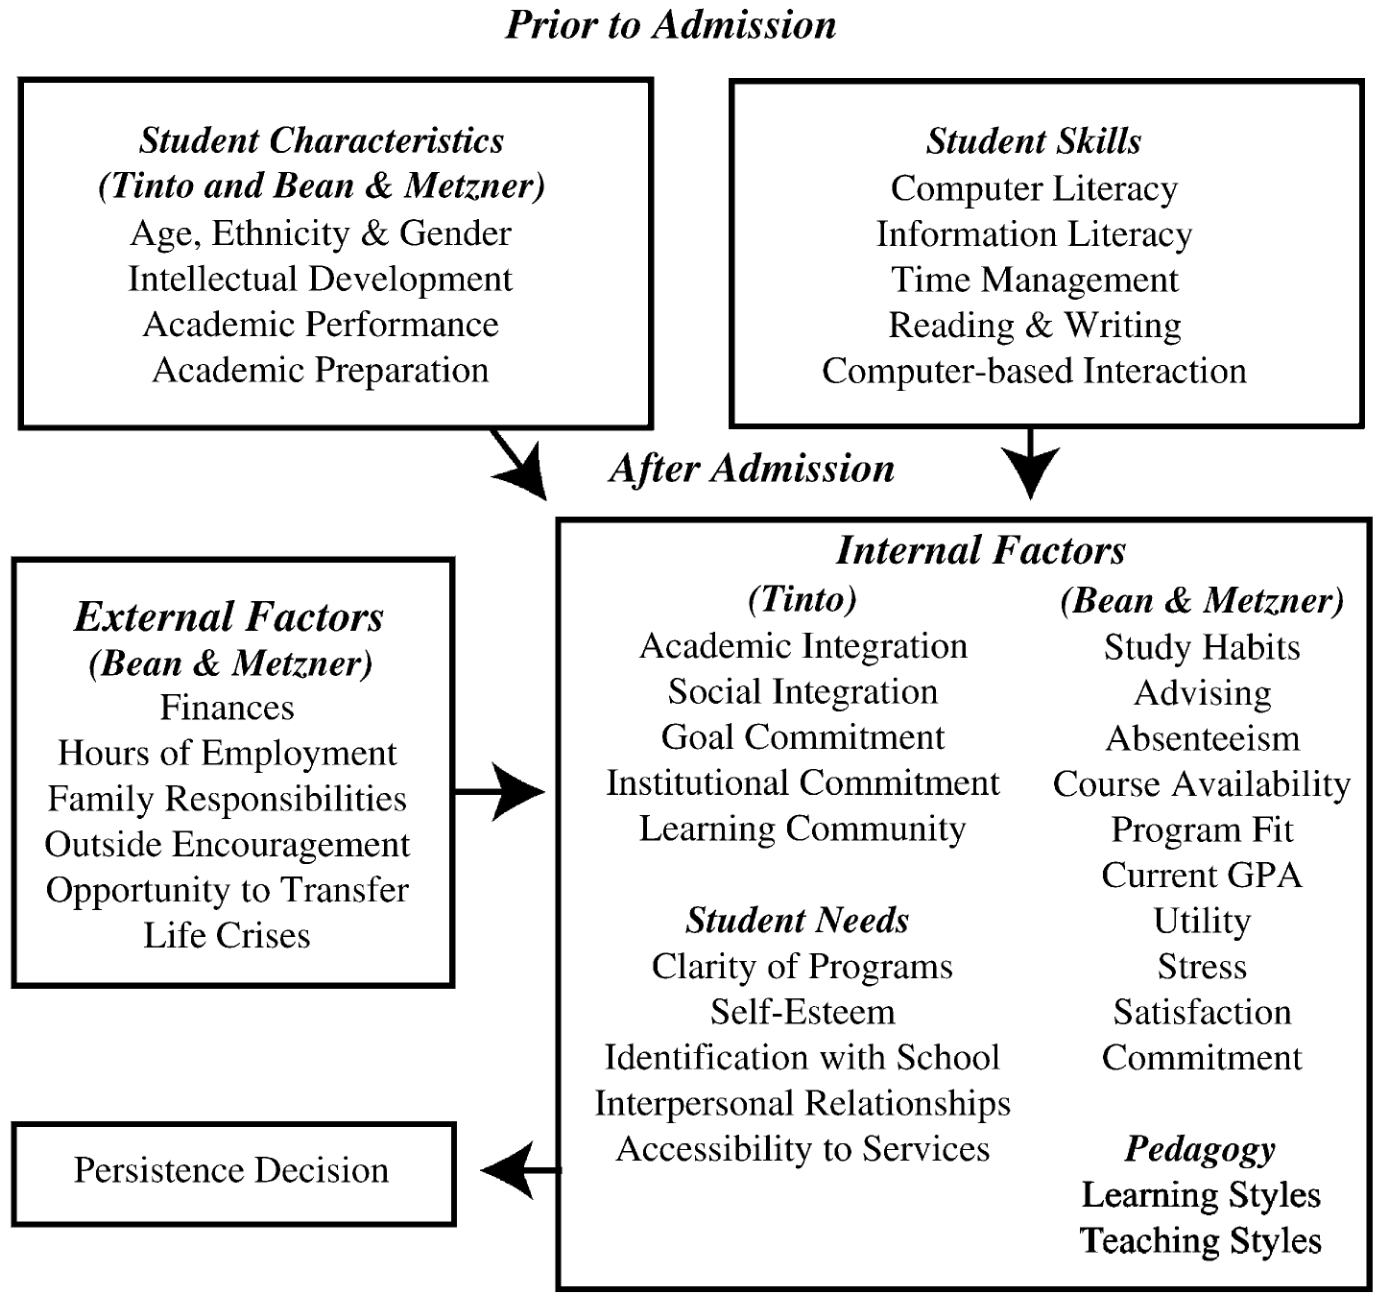
\includegraphics[width=1\linewidth]{res//diagram/composite-persistence-mdl.png}
    \caption{A composite persistence model that synthesizes the persistence models of Tinto (1975, 1987, 1993) and Bean and Metzner (1985) together with relevant research in online student skills (Rowntree, 1995; Cole, 2000) and needs (Workman \& Stenard, 1996) and the requirement to harmonize learning and teaching styles (Grow, 1996) to explain student persistence in online distance education programs. \cite{rovai_search_2003}}\cite{tinto_dropout_1975,bean_conceptual_1985,rowntree_teaching_1995}
    \label{fig:persistence-mdl}
\end{figure}

We do find similarity with our previous list of factors we have extracted from our review. Some are just more detailed version of ours that could be included in our list.

\end{document}